% Appendix B


%%%%%%%%%%%%%%%%%%%%%%%%%%%%%%%%%%%%%%%%%%%%%%%%%%%%%%%%%%%%%%%%%%%%%%
% LaTeX Overlay Generator - Annotated Figures v0.0.1
% Created with http://ff.cx/latex-overlay-generator/
%%%%%%%%%%%%%%%%%%%%%%%%%%%%%%%%%%%%%%%%%%%%%%%%%%%%%%%%%%%%%%%%%%%%%%
%\annotatedFigureBoxCustom{bottom-left}{top-right}{label}{label-position}{box-color}{label-color}{border-color}{text-color}
\newcommand*\annotatedFigureBoxCustom[8]{\draw[#5,thick,rounded corners] (#1) rectangle (#2);\node at (#4) [fill=#6,thick,shape=circle,draw=#7,inner sep=2pt,font=\sffamily,text=#8] {\textbf{#3}};}
%\annotatedFigureBox{bottom-left}{top-right}{label}{label-position}
\newcommand*\annotatedFigureBox[4]{\annotatedFigureBoxCustom{#1}{#2}{#3}{#4}{white}{white}{black}{black}}
\newcommand*\annotatedFigureText[4]{\node[draw=none, anchor=south west, text=#2, inner sep=0, text width=#3\linewidth,font=\sffamily] at (#1){#4};}
\newenvironment {annotatedFigure}[1]{\centering\begin{tikzpicture}
	\node[anchor=south west,inner sep=0] (image) at (0,0) { #1};\begin{scope}[x={(image.south east)},y={(image.north west)}]}{\end{scope}\end{tikzpicture}}
%%%%%%%%%%%%%%%%%%%%%%%%%%%%%%%%%%%%%%%%%%%%%%%%%%%%%%%%%%%%%%%%%%%%%%


\newgeometry{
	a4paper,
	top=20mm,
	bottom=10mm,
	inner=24mm,
	outer=9mm,} %bindingoffset=.5cm


\chapter{Screenshots of the game} % Main appendix title

\label{AppendixB}

\begin{figure}[h]
	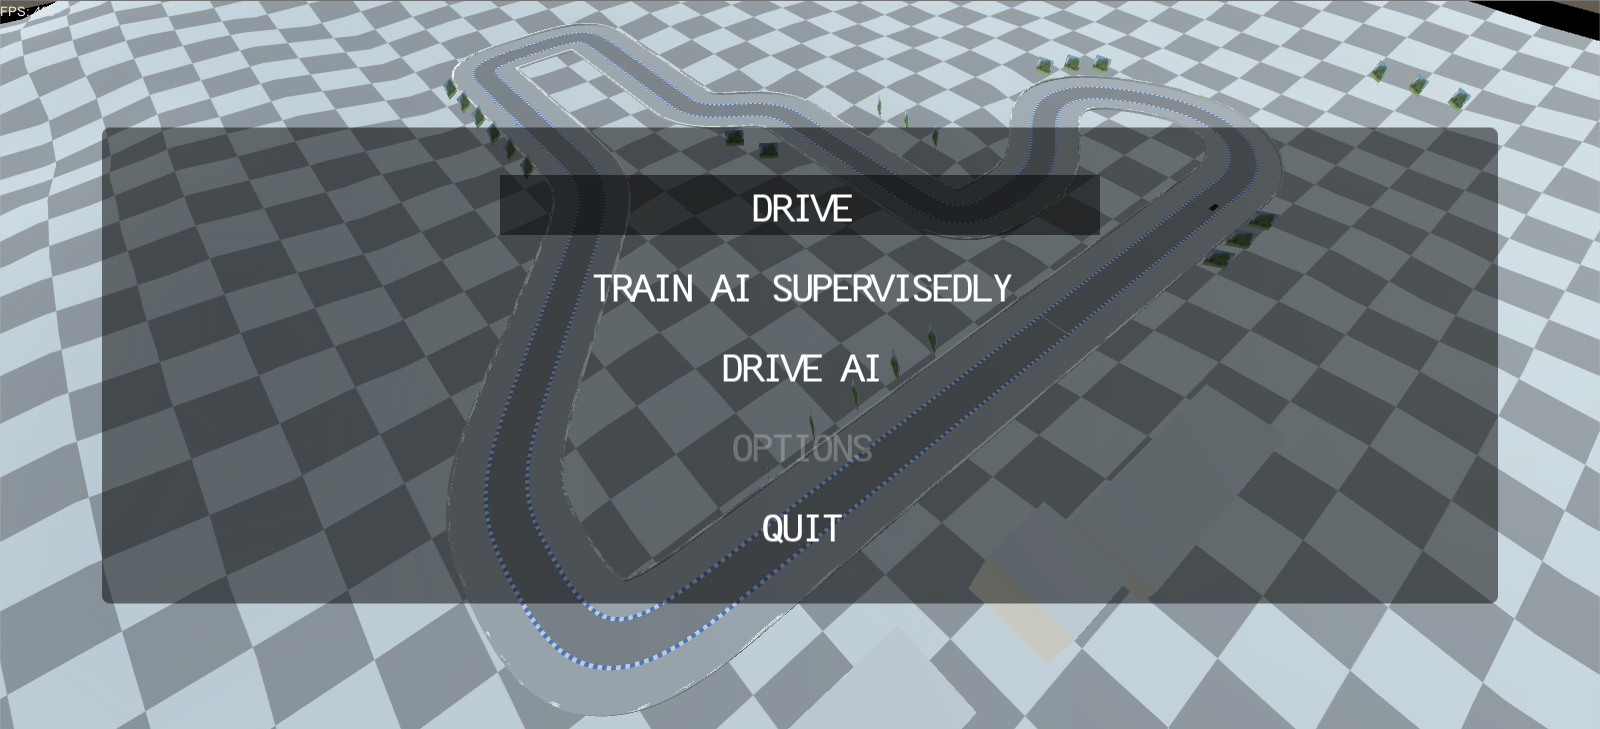
\includegraphics[width=\textwidth]{screenshot_overview}
	\centering
	\caption{Start screen / menu of the game, also showing a bird-eye view of the track}
	\label{fig:overviewshot}
\end{figure}

\begin{figure}[h]
	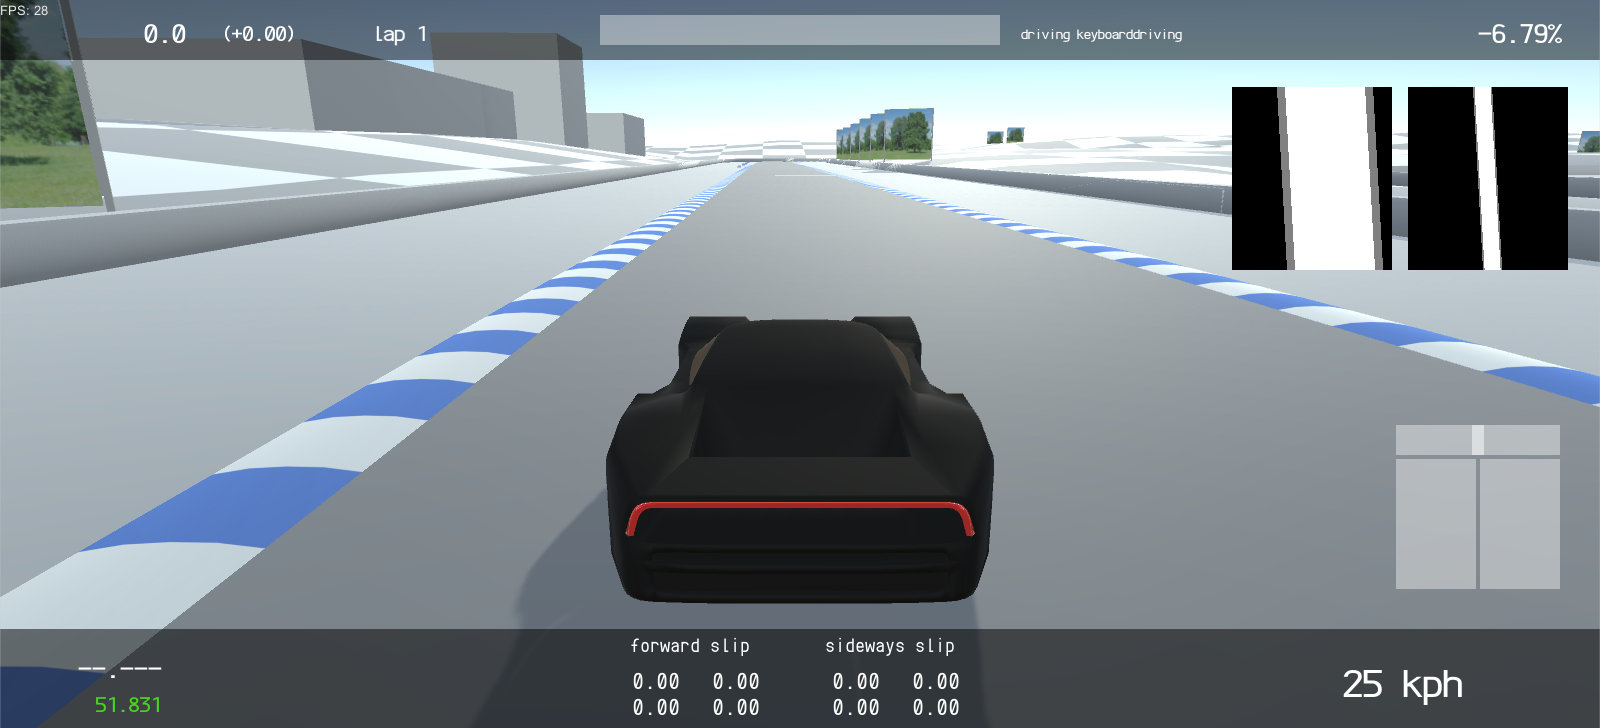
\includegraphics[width=\textwidth]{screenshot_human_juststarted}
	\centering
	\caption{\textbf{Drive} mode. For a description of the UI components, it is referred to section~\ref{ch:gamedescription}}
	\label{fig:humandriveshot}
\end{figure}

\begin{figure}[h!t]
	
	\centering
	\begin{annotatedFigure}
		{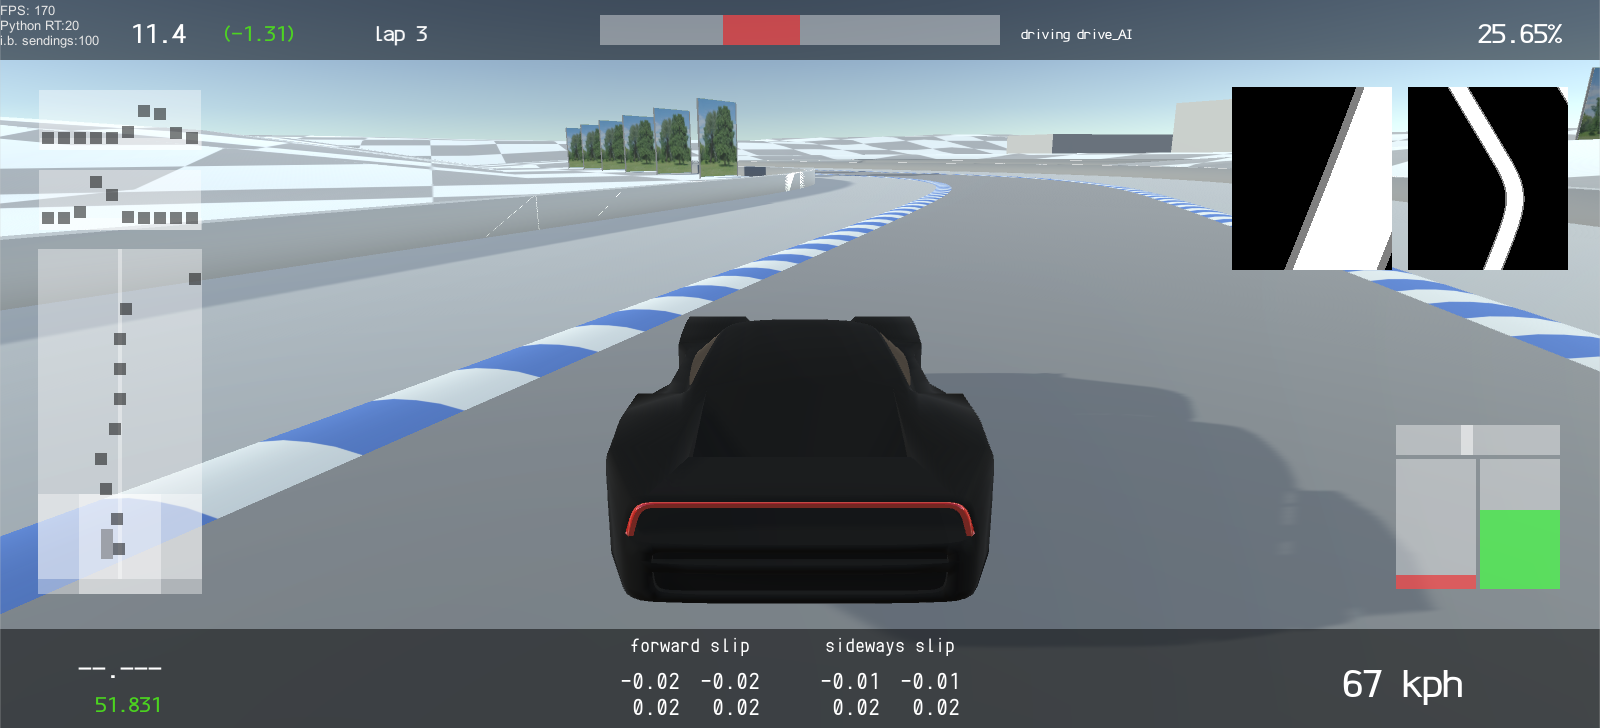
\includegraphics[width=\textwidth]{screenshot_driveAI}}
		\annotatedFigureBox{-0.002,0.9224}{0.0703,0.9951}{A}{0.0703,0.9224}%br
		\annotatedFigureBox{0.078,0.9208}{0.122,0.9813}{B}{0.122,0.9208}%br
		\annotatedFigureBox{0.1343,0.9223}{0.1946,0.9779}{C}{0.1946,0.9223}%br
		\annotatedFigureBox{0.224,0.926}{0.343,0.9769}{D}{0.343,0.926}%br
		\annotatedFigureBox{0.368,0.9295}{0.6303,0.99}{E}{0.6303,0.9295}%br
		\annotatedFigureBox{0.6363,0.9267}{0.8383,0.9823}{F}{0.8383,0.9267}%br
		\annotatedFigureBox{0.9043,0.9304}{0.989,0.9813}{G}{0.9043,0.9304}%bl
		\annotatedFigureBox{0.7663,0.6271}{0.8723,0.8937}{H}{0.7663,0.6271}%bl
		\annotatedFigureBox{0.8782,0.6231}{0.9843,0.89}{I}{0.9843,0.6231}%br
		\annotatedFigureBox{0.3743,0.1612}{0.6265,0.5963}{J}{0.6265,0.5963}%tr
		\annotatedFigureBox{0.0223,0.1963}{0.1283,0.6648}{N}{0.0223,0.1963}%bl
		\annotatedFigureBox{0.0243,0.7897}{0.1303,0.8849}{L}{0.1303,0.7897}%br
		\annotatedFigureBox{0.0222,0.6755}{0.1283,0.7713}{M}{0.1283,0.6755}%br
		\annotatedFigureBox{0.8683,0.1875}{0.981,0.4275}{K}{0.981,0.4275}%tr
		\annotatedFigureBox{0.0463,0.0073}{0.1083,0.0513}{Q}{0.1083,0.0513}%tr
		\annotatedFigureBox{0.0443,0.1656}{0.1063,0.3311}{O}{0.1063,0.1656}%br
		\annotatedFigureBox{0.3862,0.0029}{0.6083,0.1428}{R}{0.6083,0.1428}%tr
		\annotatedFigureBox{0.0443,0.0557}{0.1093,0.1153}{P}{0.1093,0.1153}%tr
		\annotatedFigureBox{0.8243,0.0293}{0.9283,0.0889}{S}{0.9283,0.0889}%tr
		\annotatedFigureBox{0.9623,0.0293}{0.9943,0.0908}{T}{0.9623,0.0908}%tl
	\end{annotatedFigure}
	
	\caption{\textbf{Drive AI} mode, showing many additional information directly on the screen. For a description of those, it is referred to sections~\ref{ch:gamedescription} and \ref{ch:thevectors}}
	\label{fig:aidriveshot}
	\begin{itemize}
		\small
		\setlength\itemsep{0.1em}
		\item \textbf{A}: Debug information. Shows FPS, the agent's response time and the time in between two sendings to the agent (the latter two only visible in \term{drive\_AI} mode).
		\item \textbf{B}: The current lap time in seconds.
		\item \textbf{C}: The time difference of the current lap in comparison to the fastest lap so far.
		\item \textbf{D}: Indicator of the current lap. Also shows if a lap is \term{invalid}.
		\item \textbf{E}: Feedback bar, graphically visualizing the time difference of only the current course section in comparison to the fastest lap so far.
		\item \textbf{F}: Indicator for the current game mode. Also indicates if QuickPause is active or if a human interferes in the \term{drive\_AI} mode.
		\item \textbf{G}: Current track progress in percent.
		\item \textbf{H}: Field of view of the first minimap-camera.
		\item \textbf{I}: Field of view of the second minimap-camera, if enabled.
		\item \textbf{J}: The car. As the main camera is fixed behind it, it will always be in this precise position.
		\item \textbf{K}: Visual representation of the values for steering (top), brake-pedal (bottom left) and throttle pedal (bottom right).
		\item \textbf{L}: Visual representation of the game's \inlinecode{progress-vector}. Only visible in \term{drive\_AI} and \term{train\_AI}.
		\item \textbf{M}: Visual representation of the game's \inlinecode{CenterDist-vector}. Only visible in \term{drive\_AI} and \term{train\_AI}.
		\item \textbf{N}: Visual representation of the game's \inlinecode{lookahead-vector}. Only visible in \term{drive\_AI} and \term{train\_AI}.
		\item \textbf{O}: Alternative representation of car's distance to the lane center. Only visible in \term{drive\_AI} and \term{train\_AI}. Overlapping with N due to low screen resolution on the machine used for the screenshot.
		\item \textbf{P}: Time needed for the last valid lap in seconds.
		\item \textbf{Q}: Time needed for the fastest valid lap (throughout different sessions) in seconds.
		\item \textbf{R}: Information about slip-behavious of the car's tires.
		\item \textbf{S}: Speed of the car in kilometers per hour.
		\item \textbf{T}: Indicates a "P" if the car is in reverse gear.
	\end{itemize}
\end{figure}

%TODO diese texte schöner, und for allem progress, centerdist und lookeahead einheitlich (nicht inlinecode? groß/klein genau wie imtext??)


